\renewcommand{\itemautorefname}{Punto}

\chapter{Modelos Propuestos} \label{Chapter:5}

Tal y como se ha comentado en la \autoref{Chapter:TransferLearning}, la explotación de las técnicas de transferencia de aprendizaje y por lo tanto el empleo de unos modelos con una serie de pesos ya definidos con respecto a un conjunto de datos determinado, constituyen la base de los sistemas propuestos en este capítulo.

\begin{figure}
    \centering
    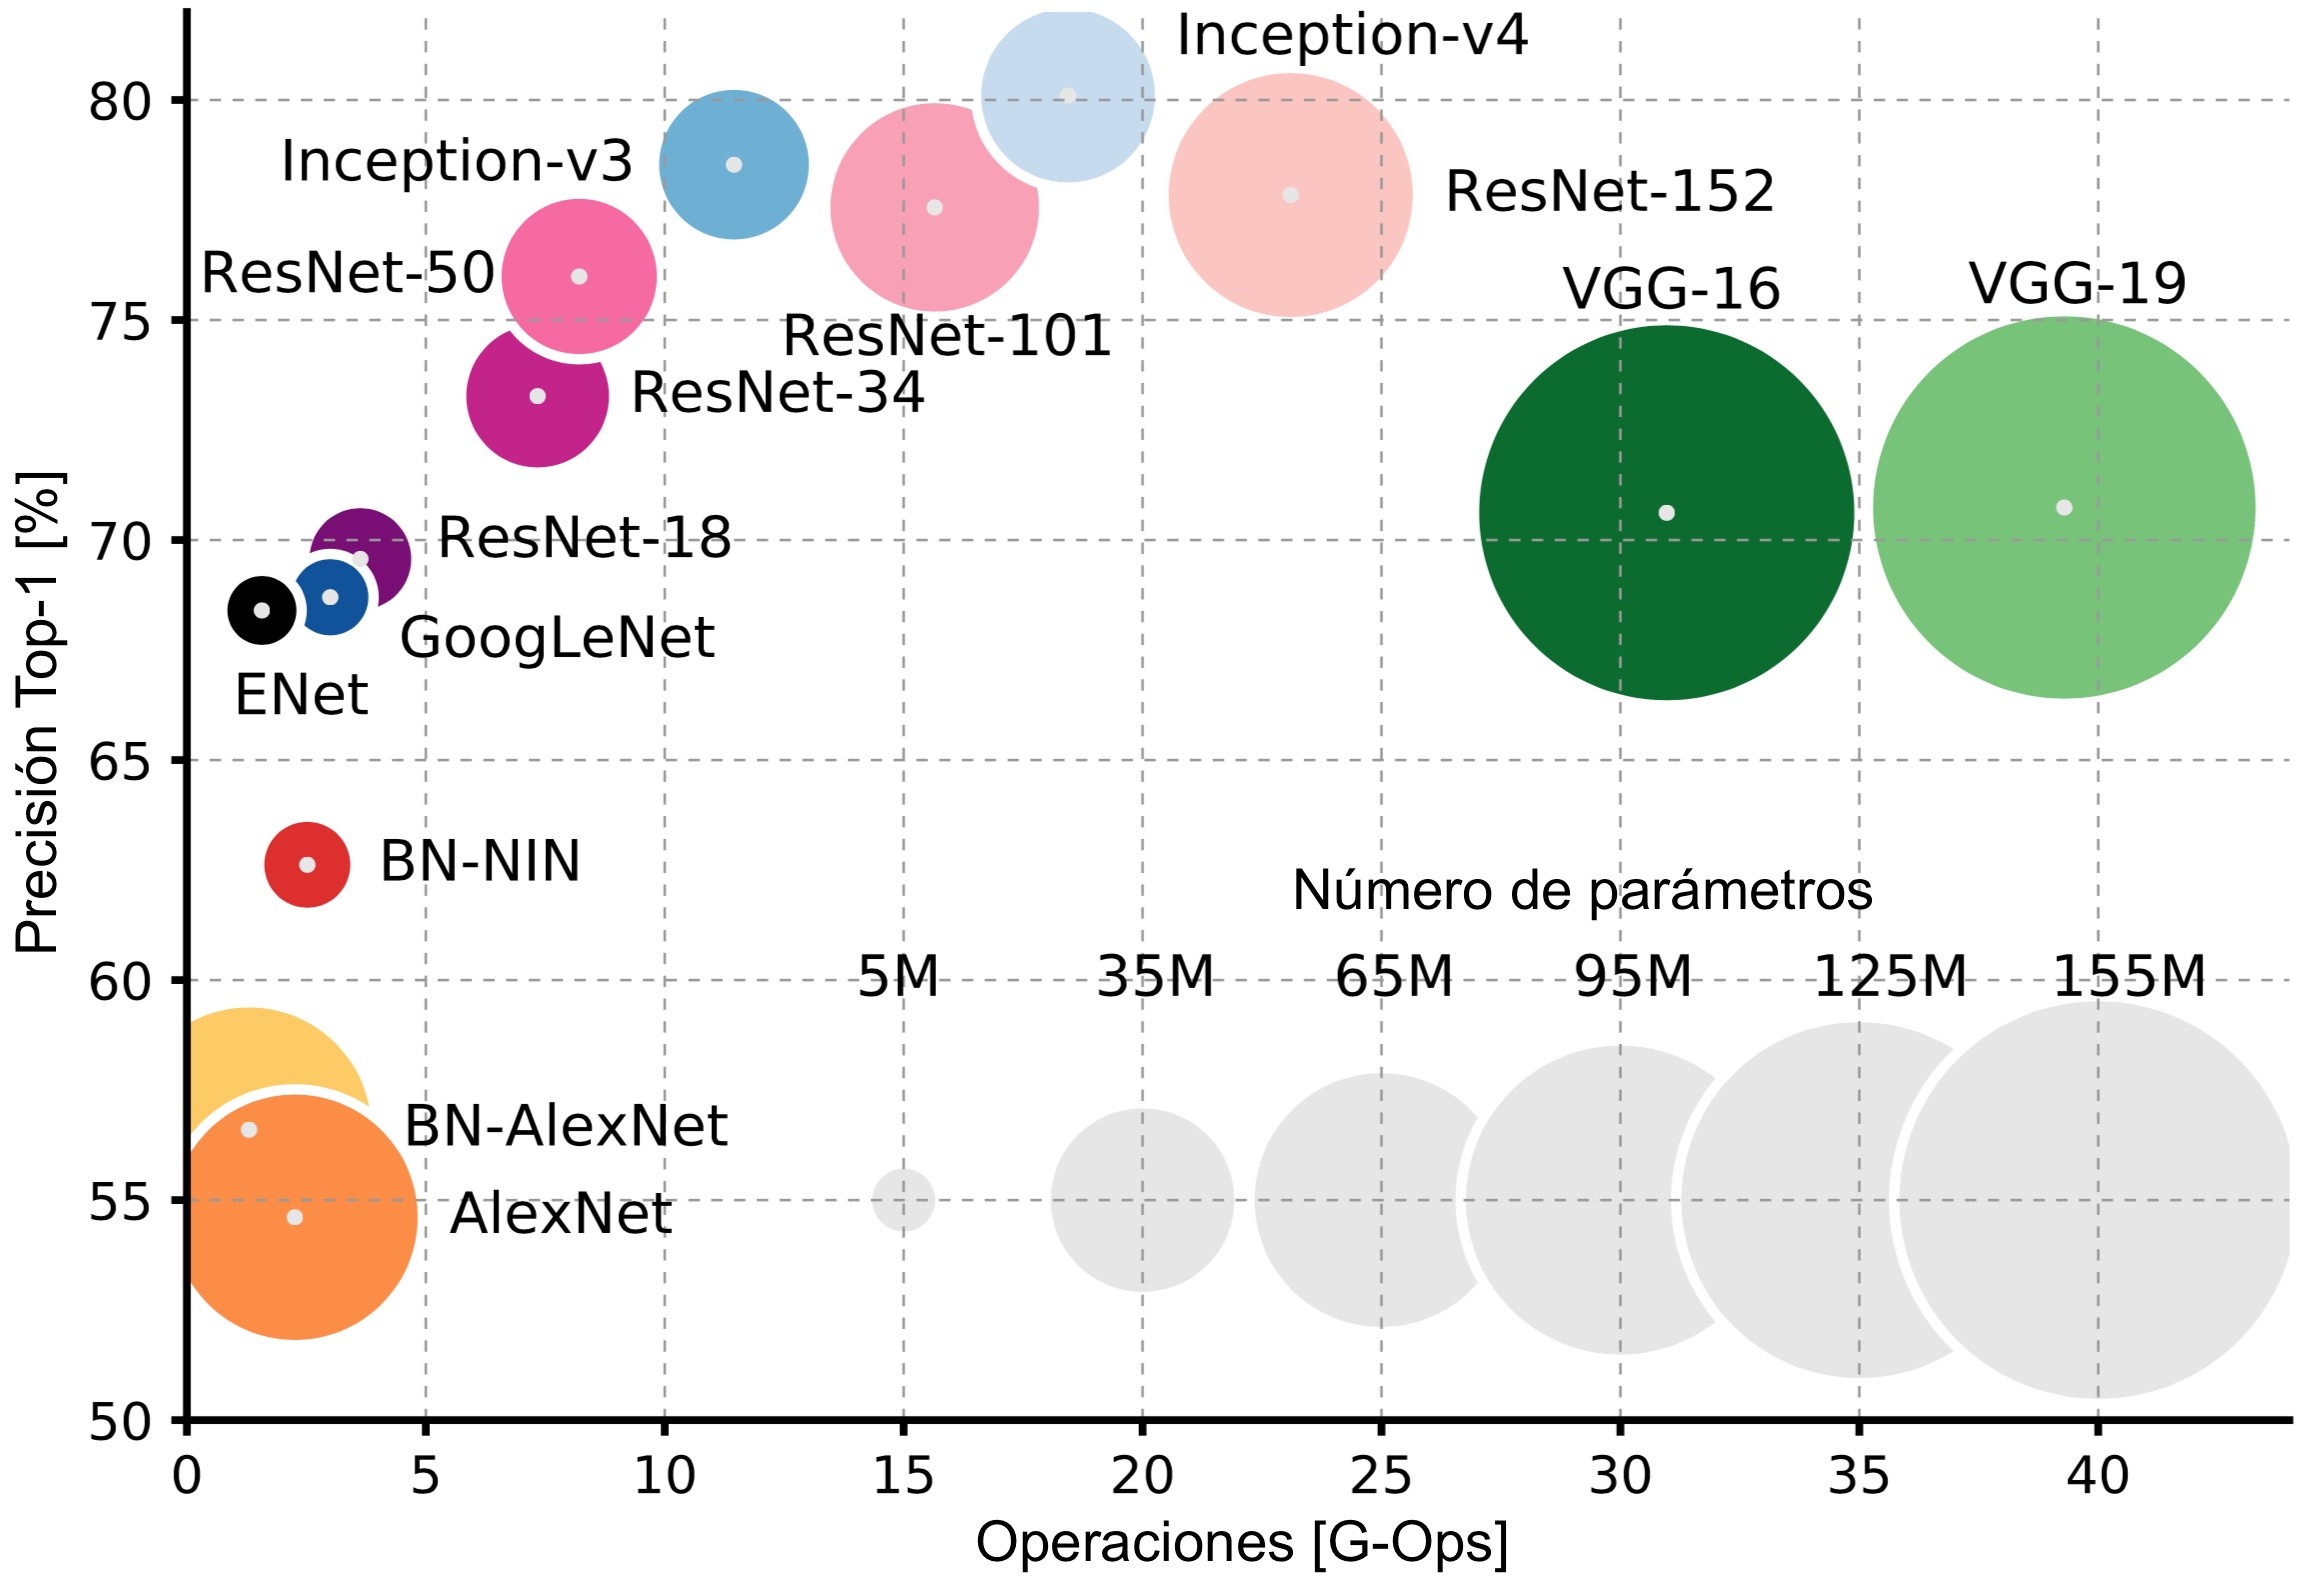
\includegraphics[scale=0.25]{Images/Models.png}
    \caption{Precisión Top-1 frente al coste computacional de una iteración del proceso de aprendizaje y el número de parámetros de la red \cite{Models}. Cabe destacar que aunque el modelo Inception-ResNet-v2 no se incluya en la figura, presenta características muy similares a Inception-v4 \cite{Inception-ResNet}.}
    \label{fig:Models}
\end{figure}

Por consiguiente, son utilizados en primera instancia los modelos Inception-v3 \cite{Inception-v3} e Inception-ResNet-v2 \cite{Inception-ResNet} con los pesos entrenados previamente sobre el conjunto de datos ImageNet descrito en la \autoref{Chapter:ImageNet}. Sin embargo, dado que las propiedades de las imágenes de esta base de datos difieren en gran medida de las características faciales que se intentan aprender y reconocer, se ha optado por explorar el uso de modelos más sencillos pero enfocados al reconocimiento facial. Es por ello que en última instancia se emplea el modelo ResNet-50 preetrenado con la base de datos VGGFace2 expuesta en la \autoref{Chapter:VGGFace2}. La comparación de estos modelos en el desempeño del desafío ILSVRC puede observarse en la \autoref{fig:Models}. Esta representación, además, escenifica la principal razón de la elección de estos modelos concretos: son los que mejores tasas obtienen con respecto al coste computacional y al número de parámetros.

Por último, obtenidos unos resultados más que aceptables y eficientes en lo que respecta al tiempo de entrenamiento, se ha intentado dar un paso más allá con la intención de mejorar las tasas de acierto y la calidad de la base de datos inicial mediante la implementación de una Red Generativa Antagónica (GAN) que permita la producción artificial de imágenes y, por lo tanto, la eliminación del desequilibrio de la distribución de clases del conjunto FER-2013.

En definitiva, a lo largo del proceso de desarrollo de un sistema de reconocimiento de expresiones faciales válido, se han ido explorando numerosas arquitecturas (Inception-v3, Inception-ResNet-v2 y ResNet-50) y técnicas (aumento de datos) con el objetivo de ir obteniendo cada vez mejores resultados sobre la base de datos FER-2013. Asimismo, a fin de permitir una comparación justa con respecto a los resultados de la \autoref{Chapter:RelatedWork}, son utilizados los protocolos de uso estipulados inicialmente por este desafío y que establecen la división de esta base de datos en tres conjuntos diferentes: entrenamiento, validación y evaluación.

\section{Afinación del Modelo Inception-v3}

Inception-v3 ha sido el resultado de las investigaciones llevadas a cabo por el equipo de Google para conseguir un modelo con una arquitectura cada vez más profunda e inteligente y capaz de desenvolverse de forma eficiente, tanto computacionalmente como cualitativamente, en el desafío ILSVR.

%Su diseño, motivado por los experimentos a gran escala llevados a cabo sobre distintas redes convolucionales, gira en torno a cuatro principios %básicos \cite{Inception-v3}:
%\begin{enumerate}
%  \item Evitar los cuellos de botella, de modo que los datos fluyan de forma uniforme a lo largo de la red.
%  \item Aumentar el número de dimensiones a medida que la información avance por la red. Las redes, de esta forma, se entrenarán más rápido.
%  \item Bajar la resolución de la entrada antes de una capa convolucional promueve un aprendizaje más rápido y no da lugar a pérdidas %significativas de la ganancia de información.
%  \item Equilibrar el ancho y la profundidad de la red aumenta el rendimiento de las redes neuronales. \label{item:4}
%\end{enumerate}

\subsection{Arquitectura}

\begin{figure}
    \centering
    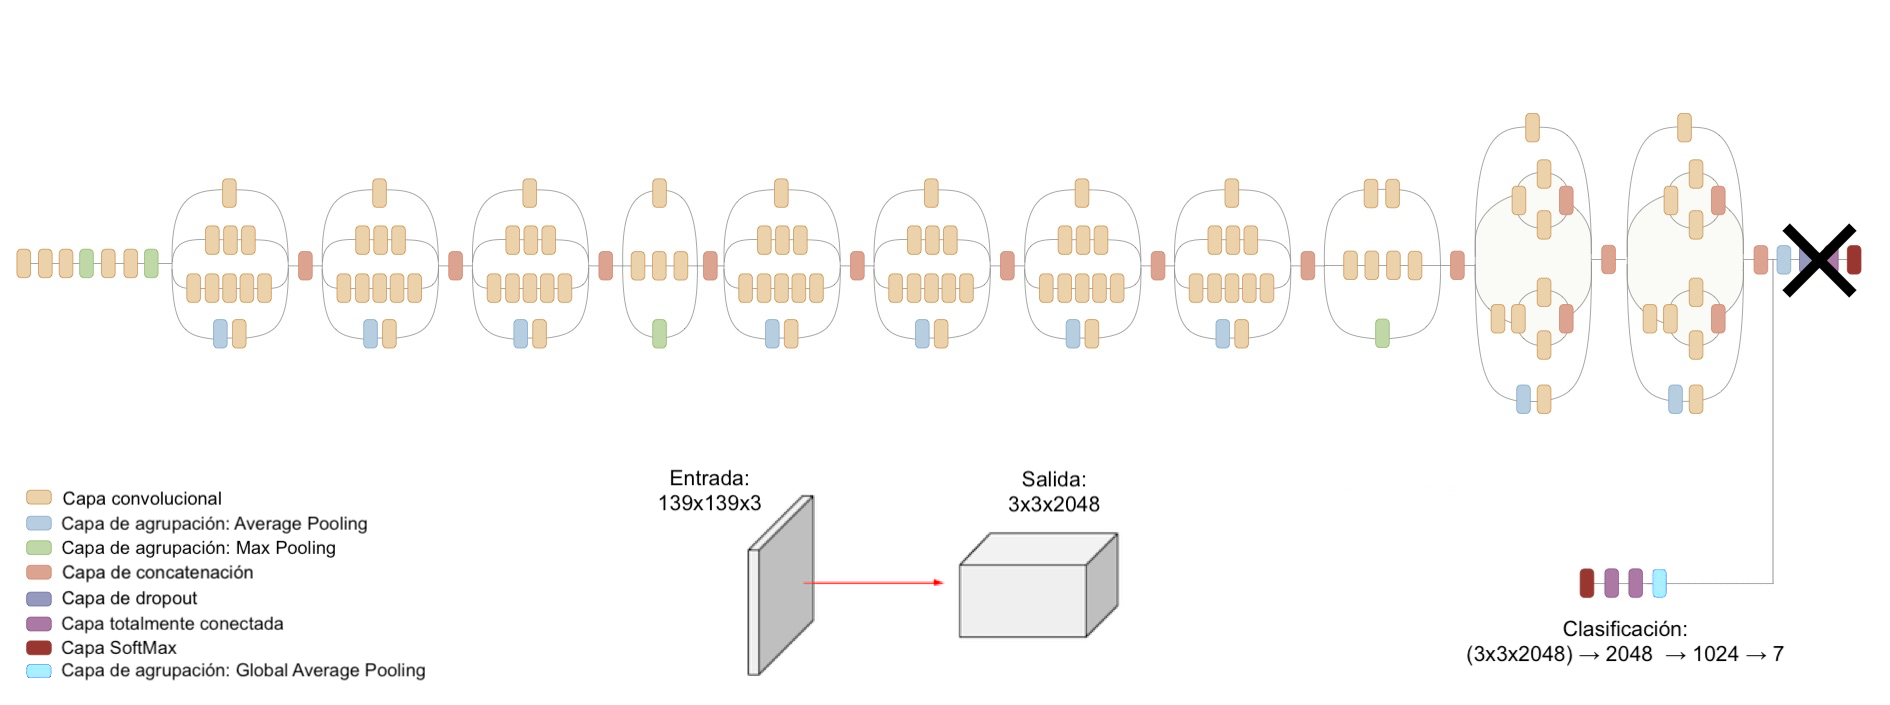
\includegraphics[width=\textwidth]{Images/Inception-v3.png}
    \caption{Arquitectura del modelo Inception-v3 adaptado al problema del reconocimiento de expresiones faciales \cite{img:Inception-v3}.}
    \label{fig:Inception-v3}
\end{figure}

\begin{figure}
    \centering
    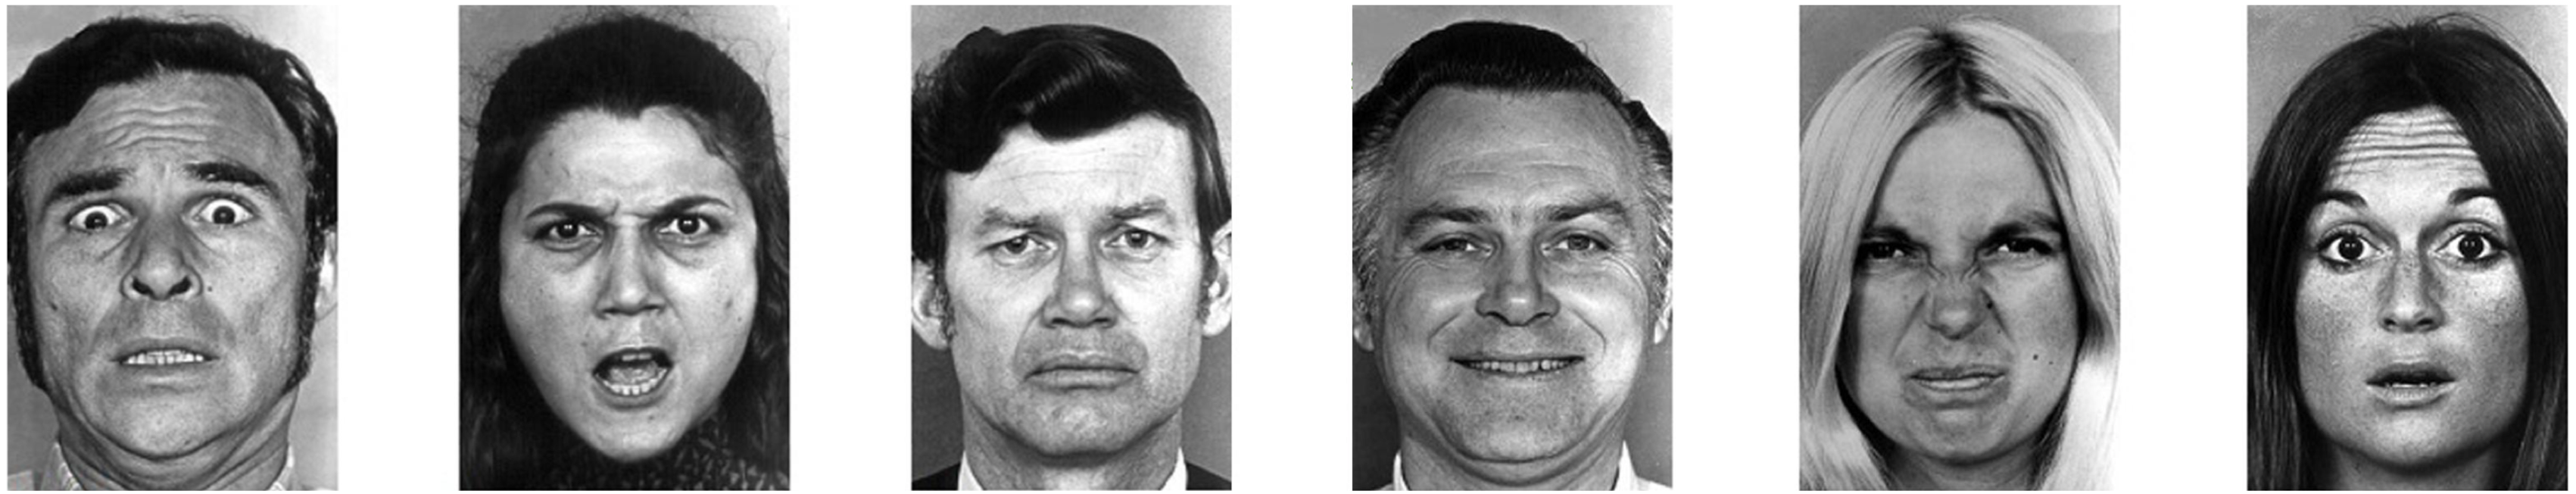
\includegraphics[width=\textwidth]{Images/emotions.png}
    \caption{\cite{Inception-v3}.}
    \label{fig:InceptionModule}
\end{figure}

En la \autoref{fig:Inception-v3} se muestra la estructura simplificada y adaptada al problema del reconocimiento de expresiones faciales del modelo Inception-v3. Esta arquitectura propuesta es básicamente una sucesión de tramos convolucionales y no linealidades, empleándose la función de activación ReLU y la normalización por lotes en cada una de las etapas, aunque esto último no se muestre explícitamente en la representación anteriormente mencionada. Como se ha podido advertir, la característica principal de este modelo es el hecho de que el flujo de datos a lo largo de algunas secciones de esta red no es secuencial, sino que se realiza en paralelo. Estas agrupaciones son conocidas como módulos Inception y representan la solución a los problemas de eficiencia de las redes estado del arte predecesoras, cumpliendo, además, la misma función y obteniendo los mismos resultados que una capa convolucional estándar. Las diferentes estructuras de estos módulos empleados por el modelo Inception-v3 pueden observarse en la \autoref{fig:InceptionModules}. La idea detrás de estas disposiciones paralelas es que dada la misma entrada para varias capas convolucionales o de agrupación de distinto tamaño se generen características únicas para cada una de ellas que posteriormente procederán a concatenarse. Este enfoque, sin embargo, da lugar a una salida con una profundidad extremadamente grande que es solucionada principalmente mediante la utilización de filtros convolucionales $1\times 1$, especialmente efectivos para reducir la dimensionalidad \cite{NetworkInNetwork}, justo antes de las capas convolucionales de mayor tamaño. Otro de los puntos que es explotado por los módulos Inception es la sustitución de los filtros tradicionales de tamaño $n\times n$ por una secuencia de capas convolucionales de dimensionest $1\times n$ y $n \times 1$. Mediante esta técnica se consigue disminuir drásticamente los costes computacionales a medida que $n$ aumenta. En la práctica y tal como se ha visto en la \autoref{fig:InceptionModules}, son utilizados básicamente filtros con $n = 7$ y $n = 3$.

Por otro lado, dado que esta red ha sido diseñada para el reto de ImageNet, ha sido necesario sustituir la etapa de clasificación del modelo Inception-v3 original, tal y como se ha visto en la \autoref{fig:Inception-v3}. De esta forma, en primer lugar se ha introducido una capa basada en la agrupación promedio global, que impone la correspondencia entre los mapas de activación y las clases, reduce el número de parámetros y además es menos propensa al sobreaprendizaje que las capas convencionales totalmente conectadas \cite{NetworkInNetwork}. Posteriormente y con la finalidad de reducir la dimensionalidad de la red de una manera suave a las 7 clases correspondientes a las expresiones faciales que se pretenden clasificar, se han insertado dos capas totalmente conectadas.

\subsection{Preprocesamiento de los datos de entrenamiento}


\subsection{Entrenamiento}

\subsection{Resultados}



\cite{Inception-v3}




\section{Afinación del Modelo Inception-ResNet-v2}

\cite{Inception-ResNet}

\subsection{Preprocesamiento de los datos}

\subsection{Arquitectura}

\subsection{Entrenamiento}

\subsection{Resultados}








\section{Afinación del Modelo ResNet-50}
\cite{ResNet}

\subsection{Preprocesamiento de los datos}

\subsection{Arquitectura}

\subsection{Entrenamiento}

\subsection{Resultados}




\section{CycleGAN - Extensión de la Base de Datos FER-2013}

\subsection{Preprocesamiento de los datos}

\subsection{Arquitectura}

\subsection{Entrenamiento}

\subsection{Resultados}